%%%%%%%%%%%%%%%%%%%%%%%%%%%%%%%%%%%%%%%%%%%%%%%%%%%%%%%%%%%%%%%%%%%%%%%%%%%%%%%
% Encoding: utf8
% Project: AIS - Exhibition ground - IS analysis and design
% Authors:
%     Libor Polčák, xpolca03@stud.fit.vutbr.cz
%     Boris Procházka, xproch63@stud.fit.vutbr.cz
%     Petr Zemek, xzemek02@stud.fit.vutbr.cz
% Description: Text of the second part of the project
%%%%%%%%%%%%%%%%%%%%%%%%%%%%%%%%%%%%%%%%%%%%%%%%%%%%%%%%%%%%%%%%%%%%%%%%%%%%%%%

\section*{Diagram případů použití}

\begin{figure}[H]
	\begin{center}
		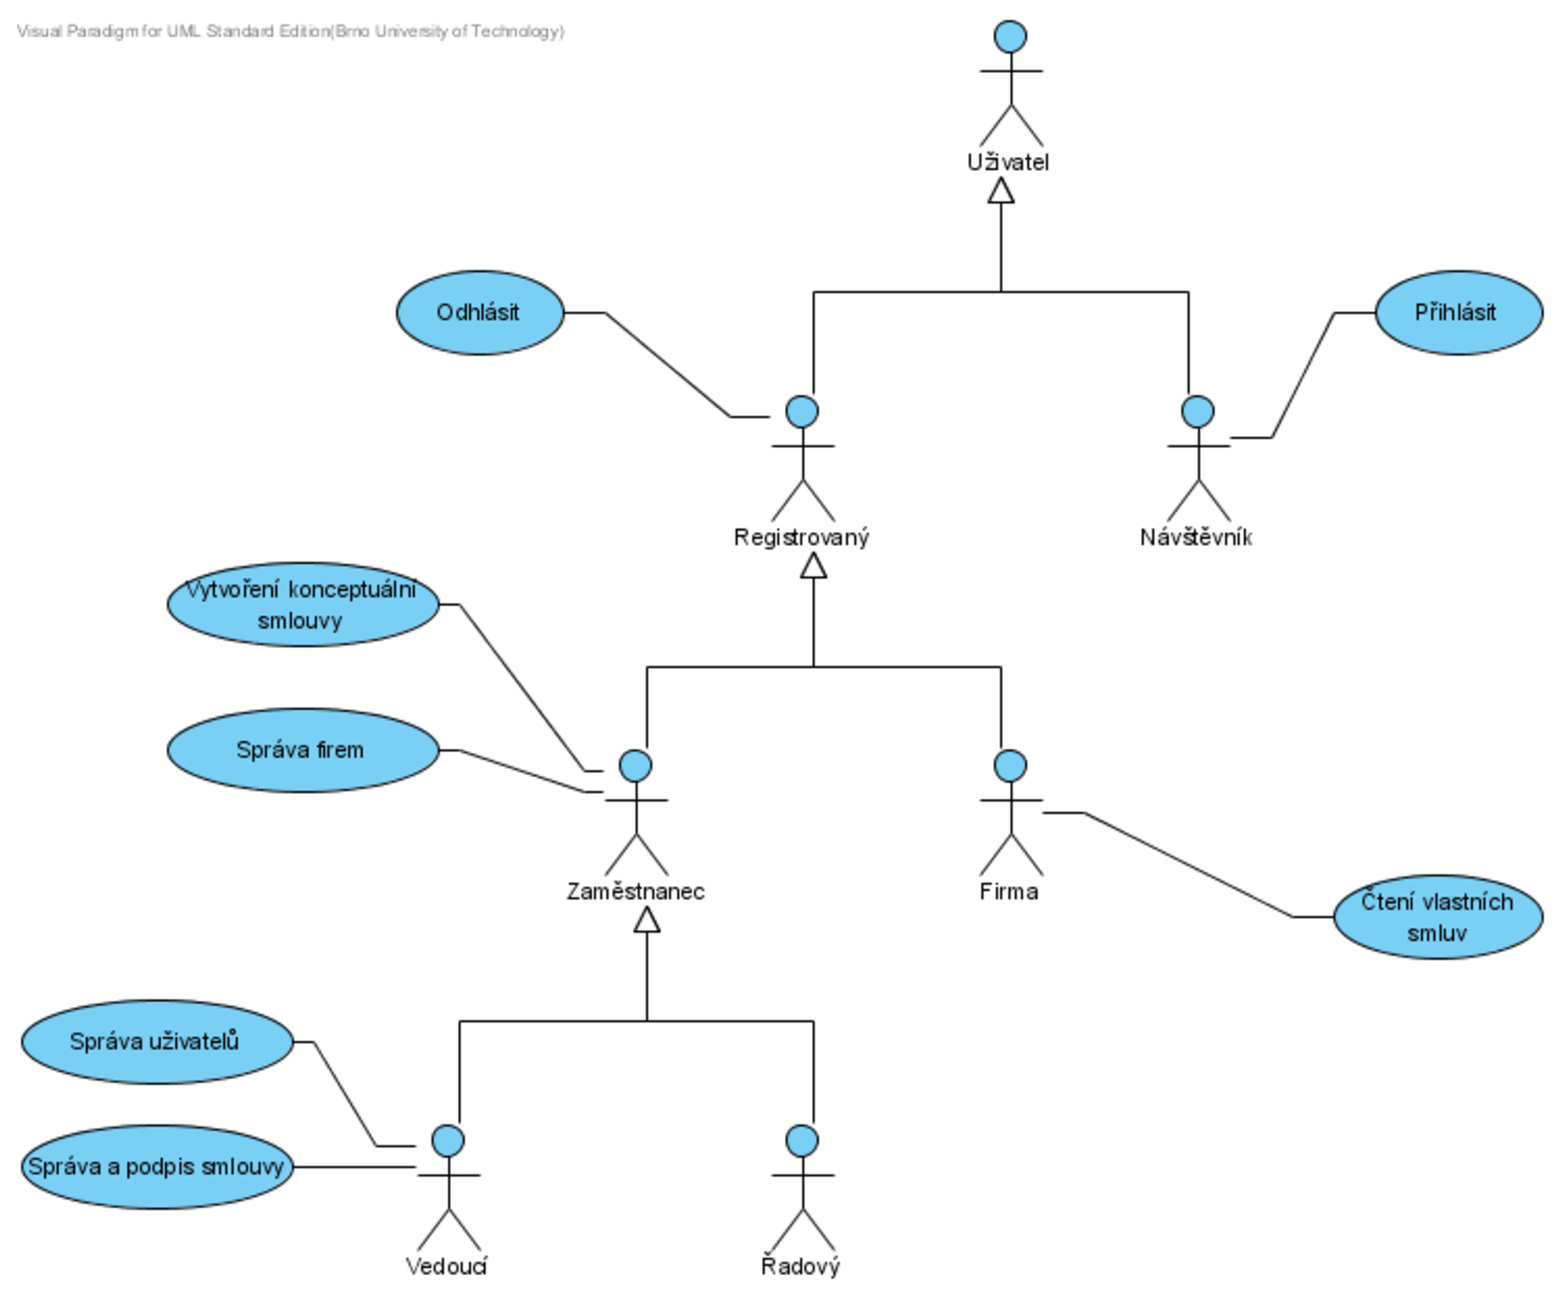
\includegraphics[width=12.5cm,keepaspectratio]{include/use_case_stage1}
	\end{center}
	\caption{Diagram případů použití}
\end{figure}

\section*{Specifikace případů použití}

\subsection*{Případ použití \uv{Přihlásit}}

\begin{ais_table}
	\hline
	Název: & Přihlásit \\

	\hline
	ID: & 1 \\

	\hline
	Stručný popis: & Uživatel se přihlašuje do systému \\

	\hline
	Primární aktéři: & Návštěvník \\

	\hline
	Sekundární aktéři: & \\

	\hline
	Předpoklady: &
		\begin{ais_table_first_enum}
			\item Uživatel není přihlášen v~systému
		\end{ais_table_first_enum} \\

	\hline
	Akce pro spuštění: & Uživatel zvolí volbu \uv{Přihlásit} \\

	\hline
	Hlavní tok: &
		\begin{ais_table_first_enum}
			\item Dokud nejsou zadány všechny přihlašovací údaje
				\begin{enumerate*}
					\item[1.1.] Uživatel zadá své přihlašovací údaje
					\item[1.2.] Uživatel potvrdí zadané údaje
				\end{enumerate*}
			\item Systém přihlásí uživatele
		\end{ais_table_first_enum} \\

	\hline
	Následné podmínky: &
		\begin{ais_table_first_enum}
			\item Uživatel je přihlášen v~systému
		\end{ais_table_first_enum} \\

	\hline
	Alternativní toky: & Nezadán některý z~přihlašovacích údajů \\
	                   & Neplatné přihlašovací údaje \\
	                   & Uživatelský účet není nastaven jako aktivní \\

	\hline
	Výjimky: & Storno \\
	         & Selhání operace \\
	         & Selhání systému \\

	\hline
\end{ais_table}

\subsubsection*{Alternativní toky případu použití \uv{Přihlásit}}

\begin{ais_table}
	\hline
	Název: & Přihlásit: Nezadán některý z~přihlašovacích údajů \\

	\hline
	ID: & 1.1 \\

	\hline
	Stručný popis: & Systém informuje uživatele, že nezadal všechny
	přihlašovací údaje \\

	\hline
	Primární aktéři: & Návštěvník \\

	\hline
	Sekundární aktéři: & \\

	\hline
	Předpoklady: &
		\begin{ais_table_first_enum}
			\item Uživatel nezadal všechny přihlašovací údaje
		\end{ais_table_first_enum} \\

	\hline
	Akce pro spuštění: & Uživatel v~kroku 1.2 hlavního toku případu užití 1
	potvrdí své přihlašovací údaje, které ale nebyly všechny zadány \\

	\hline
	Alternativní tok: &
		\begin{ais_table_first_enum}
			\item Systém uživatele upozorní, že nezadal všechny přihlašovací
			údaje
			\item Návrat k~bodu 1.1 hlavního toku
		\end{ais_table_first_enum} \\

	\hline
\end{ais_table}

\vspace{0.5cm}

\begin{ais_table}
	\hline
	Název: & Přihlásit: Neplatné přihlašovací údaje \\

	\hline
	ID: & 1.2 \\

	\hline
	Stručný popis: & Systém informuje uživatele, že zadal neplatné
	přihlašovací údaje \\

	\hline
	Primární aktéři: & Návštěvník \\

	\hline
	Sekundární aktéři: & \\

	\hline
	Předpoklady: &
		\begin{ais_table_first_enum}
			\item Uživatel zadal neplatné přihlašovací údaje
		\end{ais_table_first_enum} \\

	\hline
	Akce pro spuštění: & Uživatel v~kroku 1.2 hlavního toku případu užití 1
	potvrdí své přihlašovací údaje, které jsou ale neplatné \\

	\hline
	Alternativní tok: &
		\begin{ais_table_first_enum}
			\item Systém uživatele upozorní, že zadal neplatné přihlašovací
			údaje
			\item Návrat k~bodu 1.1 hlavního toku
		\end{ais_table_first_enum} \\

	\hline
\end{ais_table}

\begin{ais_table}
	\hline
	Název: & Přihlásit: Uživatelský účet není nastaven jako aktivní  \\

	\hline
	ID: & 1.2 \\

	\hline
	Stručný popis: & Systém informuje uživatele, že zadal neplatné
	přihlašovací údaje \\

	\hline
	Primární aktéři: & Návštěvník \\

	\hline
	Sekundární aktéři: & \\

	\hline
	Předpoklady: &
		\begin{ais_table_first_enum}
			\item Uživatelský účet, ke kterému se návštěvník přihlašuje,
				není nastaven jako aktivní
		\end{ais_table_first_enum} \\

	\hline
	Akce pro spuštění: & Uživatel v~kroku 1.2 hlavního toku případu užití 1
	potvrdí své přihlašovací údaje, které ale patří k~účtu, který není nastaven
	jako aktivní \\

	\hline
	Alternativní tok: &
		\begin{ais_table_first_enum}
			\item Systém uživatele upozorní, že zadal neplatné přihlašovací
				údaje (z~bezpečnostních důvodů se nerozlišuje mezi situací,
				kdy opravdu zadal neplatné údaje, a situací, kdy není účet nastaven
				jako aktivní)
			\item Návrat k~bodu 1.1 hlavního toku
		\end{ais_table_first_enum} \\

	\hline
\end{ais_table}

\subsubsection*{Výjimky případu použití \uv{Přihlásit}}

\begin{ais_table}
	\hline
	Název: & Přihlásit: Storno \\

	\hline
	ID: & 1.E.1 \\

	\hline
	Stručný popis: & Uživatel ukončí případ použití \\

	\hline
	Primární aktéři: & Návštěvník \\

	\hline
	Sekundární aktéři: & \\

	\hline
	Předpoklady: &
		\begin{ais_table_first_enum}
			\item Žádné
		\end{ais_table_first_enum} \\

	\hline
	Akce pro spuštění: & Uživatel zvolí storno kdykoliv v~průběhu hlavního toku
	případu užití \\

	\hline
	Tok: &
		\begin{ais_table_first_enum}
			\item Systém vrátí uživatele do místa, odkud vyvolal případ použití
		\end{ais_table_first_enum} \\

	\hline
	Následné podmínky: &
		\begin{ais_table_first_enum}
			\item Uživatel nebyl přihlášen
		\end{ais_table_first_enum} \\

	\hline
\end{ais_table}

\vspace{0.5cm}

\begin{ais_table}
	\hline
	Název: & Přihlásit: Selhání operace \\

	\hline
	ID: & 1.E.2 \\

	\hline
	Stručný popis: & Systém nedokáže pokračovat v~případu užití a ukončí ho \\

	\hline
	Primární aktéři: & Návštěvník nebo systém \\

	\hline
	Sekundární aktéři: & \\

	\hline
	Předpoklady: &
		\begin{ais_table_first_enum}
			\item Systém neprovedl korektně některý krok hlavního toku
		\end{ais_table_first_enum} \\

	\hline
	Akce pro spuštění: & Selhání v~libovolném místě hlavního toku případu užití
	1 \\

	\hline
	Tok: &
		\begin{ais_table_first_enum}
			\item Systém informuje uživatele o~selhání
			\item Systém vrátí uživatele do místa, dokud vyvolal případ použití
		\end{ais_table_first_enum} \\

	\hline
	Následné podmínky: &
		\begin{ais_table_first_enum}
			\item Uživatel nebyl přihlášen
		\end{ais_table_first_enum} \\

	\hline
\end{ais_table}

\vspace{0.5cm}

\begin{ais_table}
	\hline
	Název: & Přihlásit: Selhání systému \\

	\hline
	ID: & 1.E.3 \\

	\hline
	Stručný popis: & Systém nedokáže pokračovat v~činnosti \\

	\hline
	Primární aktéři: & Návštěvník nebo systém \\

	\hline
	Sekundární aktéři: & \\

	\hline
	Předpoklady: &
		\begin{ais_table_first_enum}
			\item Systém nemůže pokračovat v~činnosti
		\end{ais_table_first_enum} \\

	\hline
	Akce pro spuštění: & Selhání v~libovolném místě hlavního toku případu užití
	1 \\

	\hline
	Tok: &
		\begin{ais_table_first_enum}
			\item Systém informuje uživatele o~selhání
			\item Systém je ukončen
		\end{ais_table_first_enum} \\

	\hline
	Následné podmínky: &
		\begin{ais_table_first_enum}
			\item Uživatel nebyl přihlášen
			\item Systém je ukončen
		\end{ais_table_first_enum} \\

	\hline
\end{ais_table}

\subsection*{Případ použití \uv{Podpis smlouvy}}

\begin{ais_table}
	\hline
	Název: & Podpis smlouvy \\

	\hline
	ID: & 2 \\

	\hline
	Stručný popis: & Oprávněný uživatel (vedoucí) podepíše obsah smlouvy\\

	\hline
	Primární aktéři: & Vedoucí \\

	\hline
	Sekundární aktéři: & \\

	\hline
	Předpoklady: &
		\begin{ais_table_first_enum}
			\item Uživatel je přihlášen do systému jako vedoucí
			\item Uživatel má zobrazenou existující nepodepsanou smlouvu
			\item Smlouva obsahuje datum splatnosti a neprázdný text smlouvy
		\end{ais_table_first_enum} \\

	\hline
	Akce pro spuštění: & Uživatel zvolí volbu \uv{Podepsat smlouvu} \\

	\hline
	Hlavní tok: &
		\begin{ais_table_first_enum}
			\item Nastaví se datum uzavření smlouvy podle aktuálního data
			\item Přiřaď přihlášeného uživatele ke smlouvě jako signatáře
		\end{ais_table_first_enum} \\

	\hline
	Následné podmínky: &
		\begin{ais_table_first_enum}
			\item Smlouva byla podepsána
		\end{ais_table_first_enum} \\

	\hline
	Alternativní toky: & Žádné \\

	\hline
	Výjimky: & Selhání operace \\
	         & Selhání systému \\

	\hline
\end{ais_table}

\subsubsection*{Výjimky případu použití \uv{Podpis smlouvy}}

Výjimky případu použití \uv{Podpis smlouvy} odpovídají (po úpravách) výjimkám
případu použití 1.

\subsection*{Případ použití \uv{Správa firmy}}

\begin{ais_table}
	\hline
	Název: & Správa firmy\\

	\hline
	ID: & 3\\

	\hline
	Stručný popis: & Zaměstnanec (ať již řadový či vedoucí) spravuje (akce čti, přidej, uprav a zruš) jednotlivé firmy\\

	\hline
	Primární aktéři: & Zaměstnanec\\

	\hline
	Sekundární aktéři: & \\

	\hline
	Předpoklady: &
		\begin{ais_table_first_enum}
			\item Uživatel je přihlášen do systému jako zaměstnanec
			\item Pro akce čti, uprav a zruš musí firma existovat v~systému
		\end{ais_table_first_enum} \\

	\hline
	Akce pro spuštění: & Zaměstnanec zvolí volbu \uv{zobraz firmu}, \uv{přidej firmu}, \uv{uprav firmu} či \uv{smaž firmu} \\

	\hline
	Hlavní tok: &
		\begin{ais_table_first_enum}
			\item Pro akce čti, uprav a zruš jsou informace o~firmě načteny ze systému
			\item Pro akce čti, uprav a zruš jsou načtené informace zobrazeny. Pro akci přidej se zobrazí prázdný formulář
			\item Pro akce přidej a uprav jsou zobrazené informace editovatelné
			\item Pro akce přidej a uprav prováděj dokud nejsou zadané údaje platné
				\begin{enumerate*}
					\item[4.1.] Zaměstnanec přidává či upravuje údaje o~firmě
					\item[4.2.] Systém ověří správnost zadaných údajů
				\end{enumerate*}
			\item Pro akce přidej, uprav a zruš jsou informace o~firmě zaslány systému ke zpracování
		\end{ais_table_first_enum} \\

	\hline
	Následné podmínky: &
		\begin{ais_table_first_enum}
			\item Pro akce přidej, uprav a zruš jsou změny promítnuty do systému
		\end{ais_table_first_enum} \\

	\hline
	Alternativní toky: & Nezadán některý z~firemních údajů \\
	                   & Neplatné firemní údaje\\

	\hline
	Výjimky: & Storno \\
	         & Selhání operace \\
	         & Selhání systému \\

	\hline
\end{ais_table}

\subsubsection*{Alternativní toky a výjimky případu použití \uv{Správa firmy}}

Alternativní toky a výjimky případu použití \uv{Správa firmy} odpovídají (po
úpravách) alternativním tokům a výjimkám případu použití 1.

\pagebreak

\section*{Konceptuální diagram tříd}

\begin{figure}[H]
	\begin{center}
		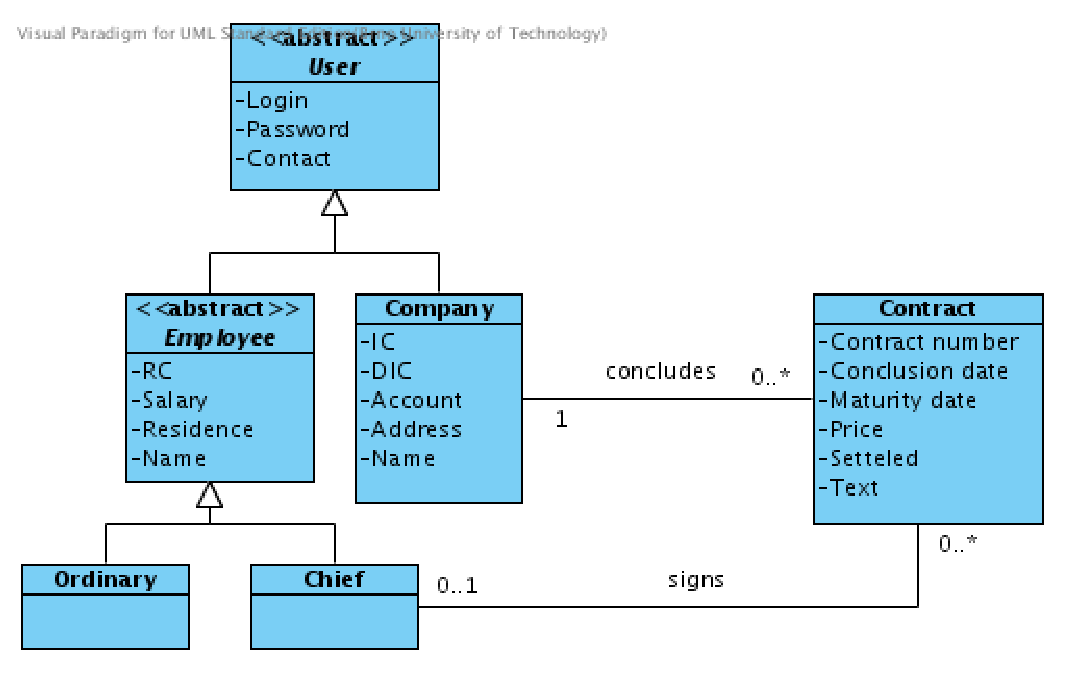
\includegraphics[width=9cm,keepaspectratio]{include/conceptual_stage1}
	\end{center}
	\caption{Konceptuální diagram tříd}
	\label{fig:ConceptualStage1}
\end{figure}

\pagebreak

\section*{Návrh schématu databáze}

\begin{figure}[H]
	\begin{center}
		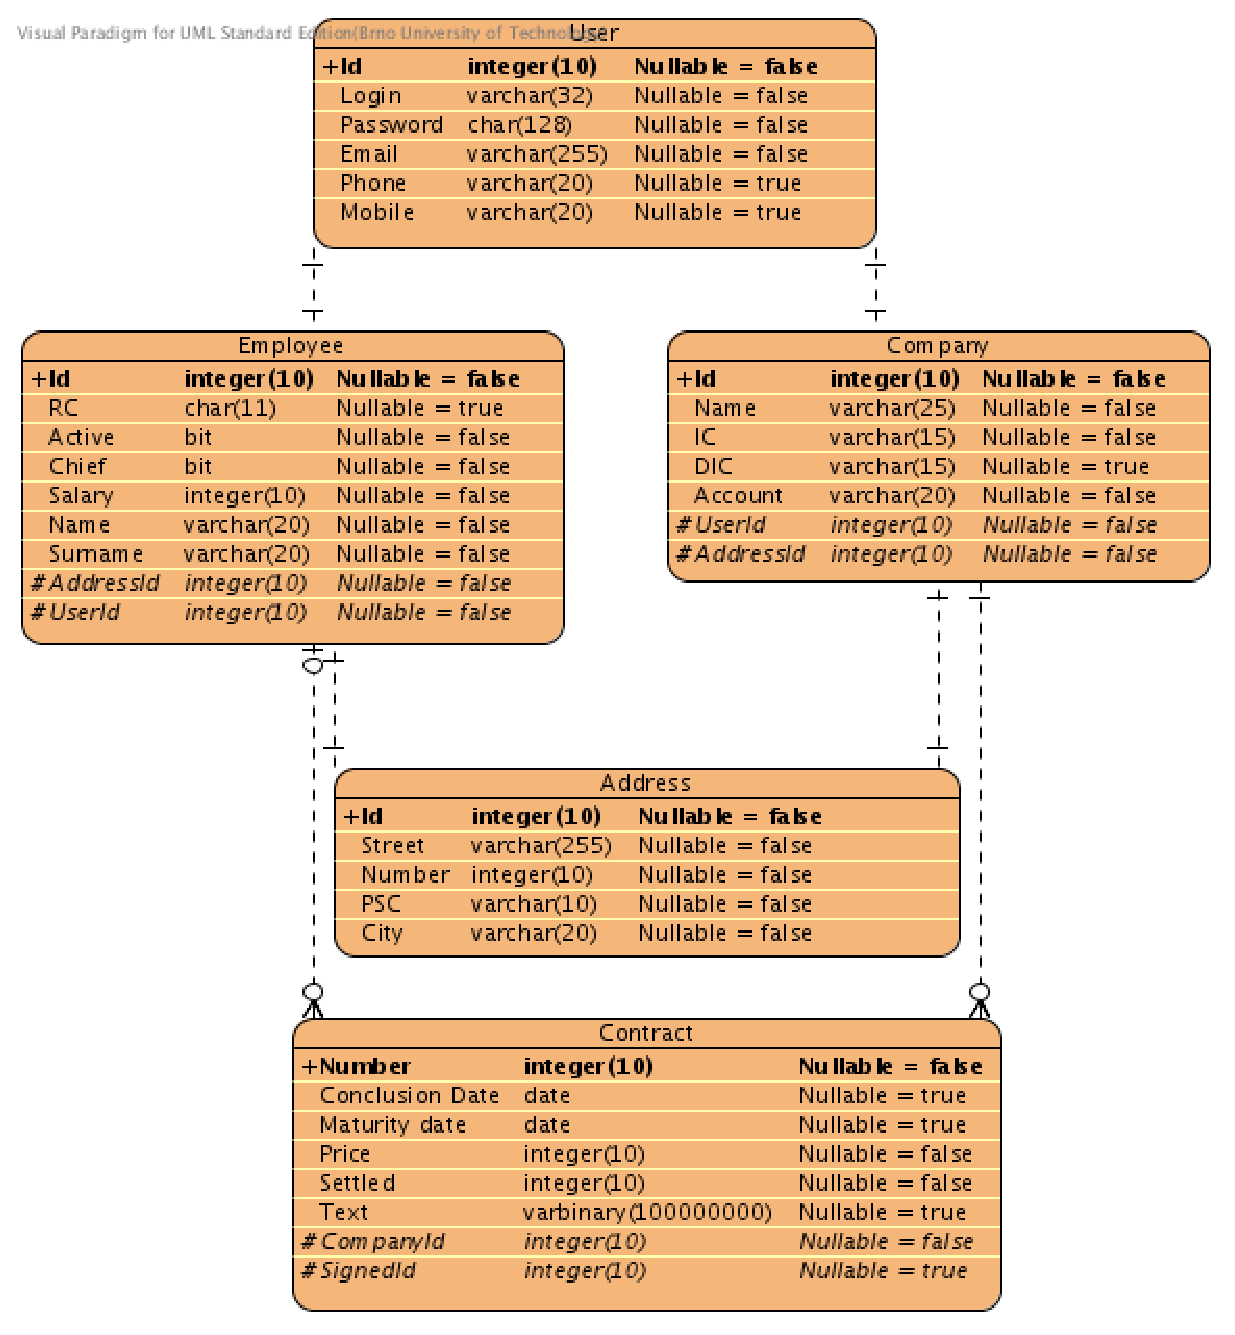
\includegraphics[width=10cm,keepaspectratio]{include/schema_stage1}
	\end{center}
	\caption{Návrh schématu databáze}
	\label{fig:SchemaStage1}
\end{figure}

\pagebreak

\section*{Návrh architektury aplikace}

Byla použita architektura PCMEF.

\begin{figure}[H]
	\begin{center}
		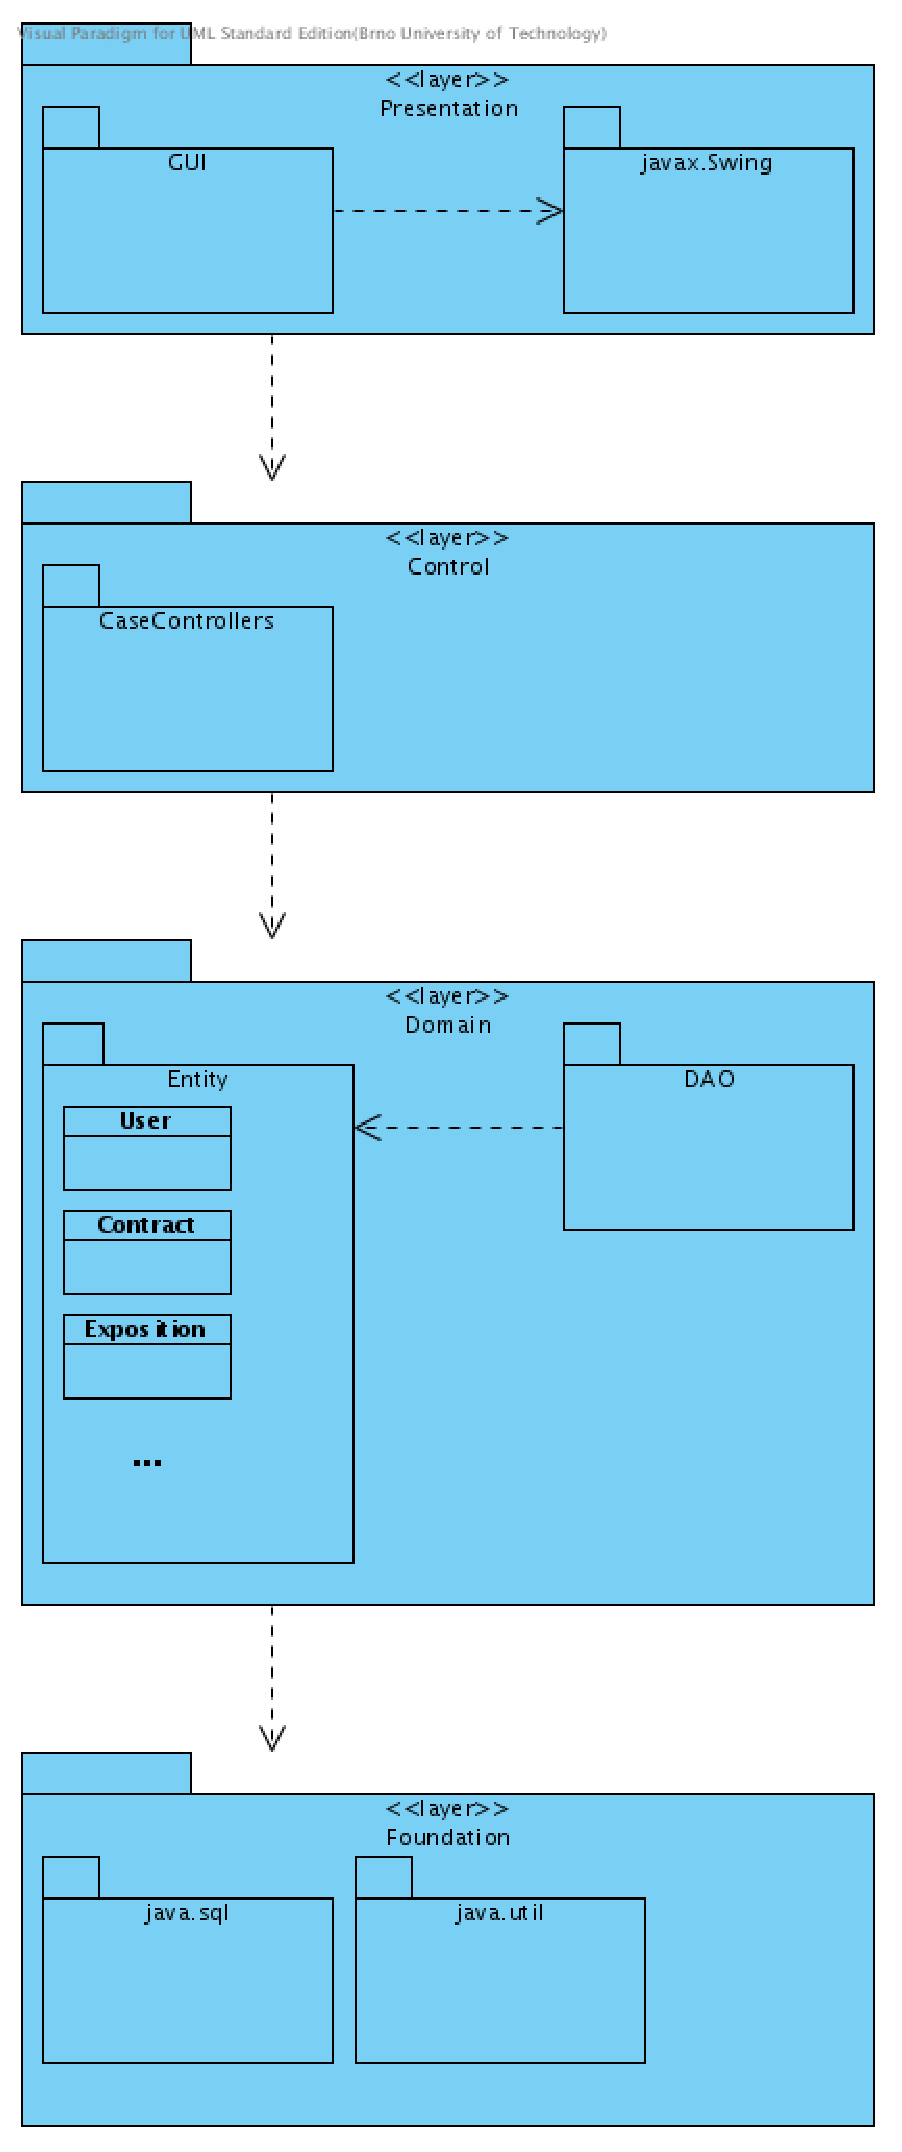
\includegraphics[width=7.5cm,keepaspectratio]{include/architecture}
	\end{center}
	\caption{Návrh architektury aplikace}
	\label{fig:Architecture}
\end{figure}

\pagebreak

\section*{Diagram návrhových tříd}

\begin{figure}[H]
	\begin{center}
		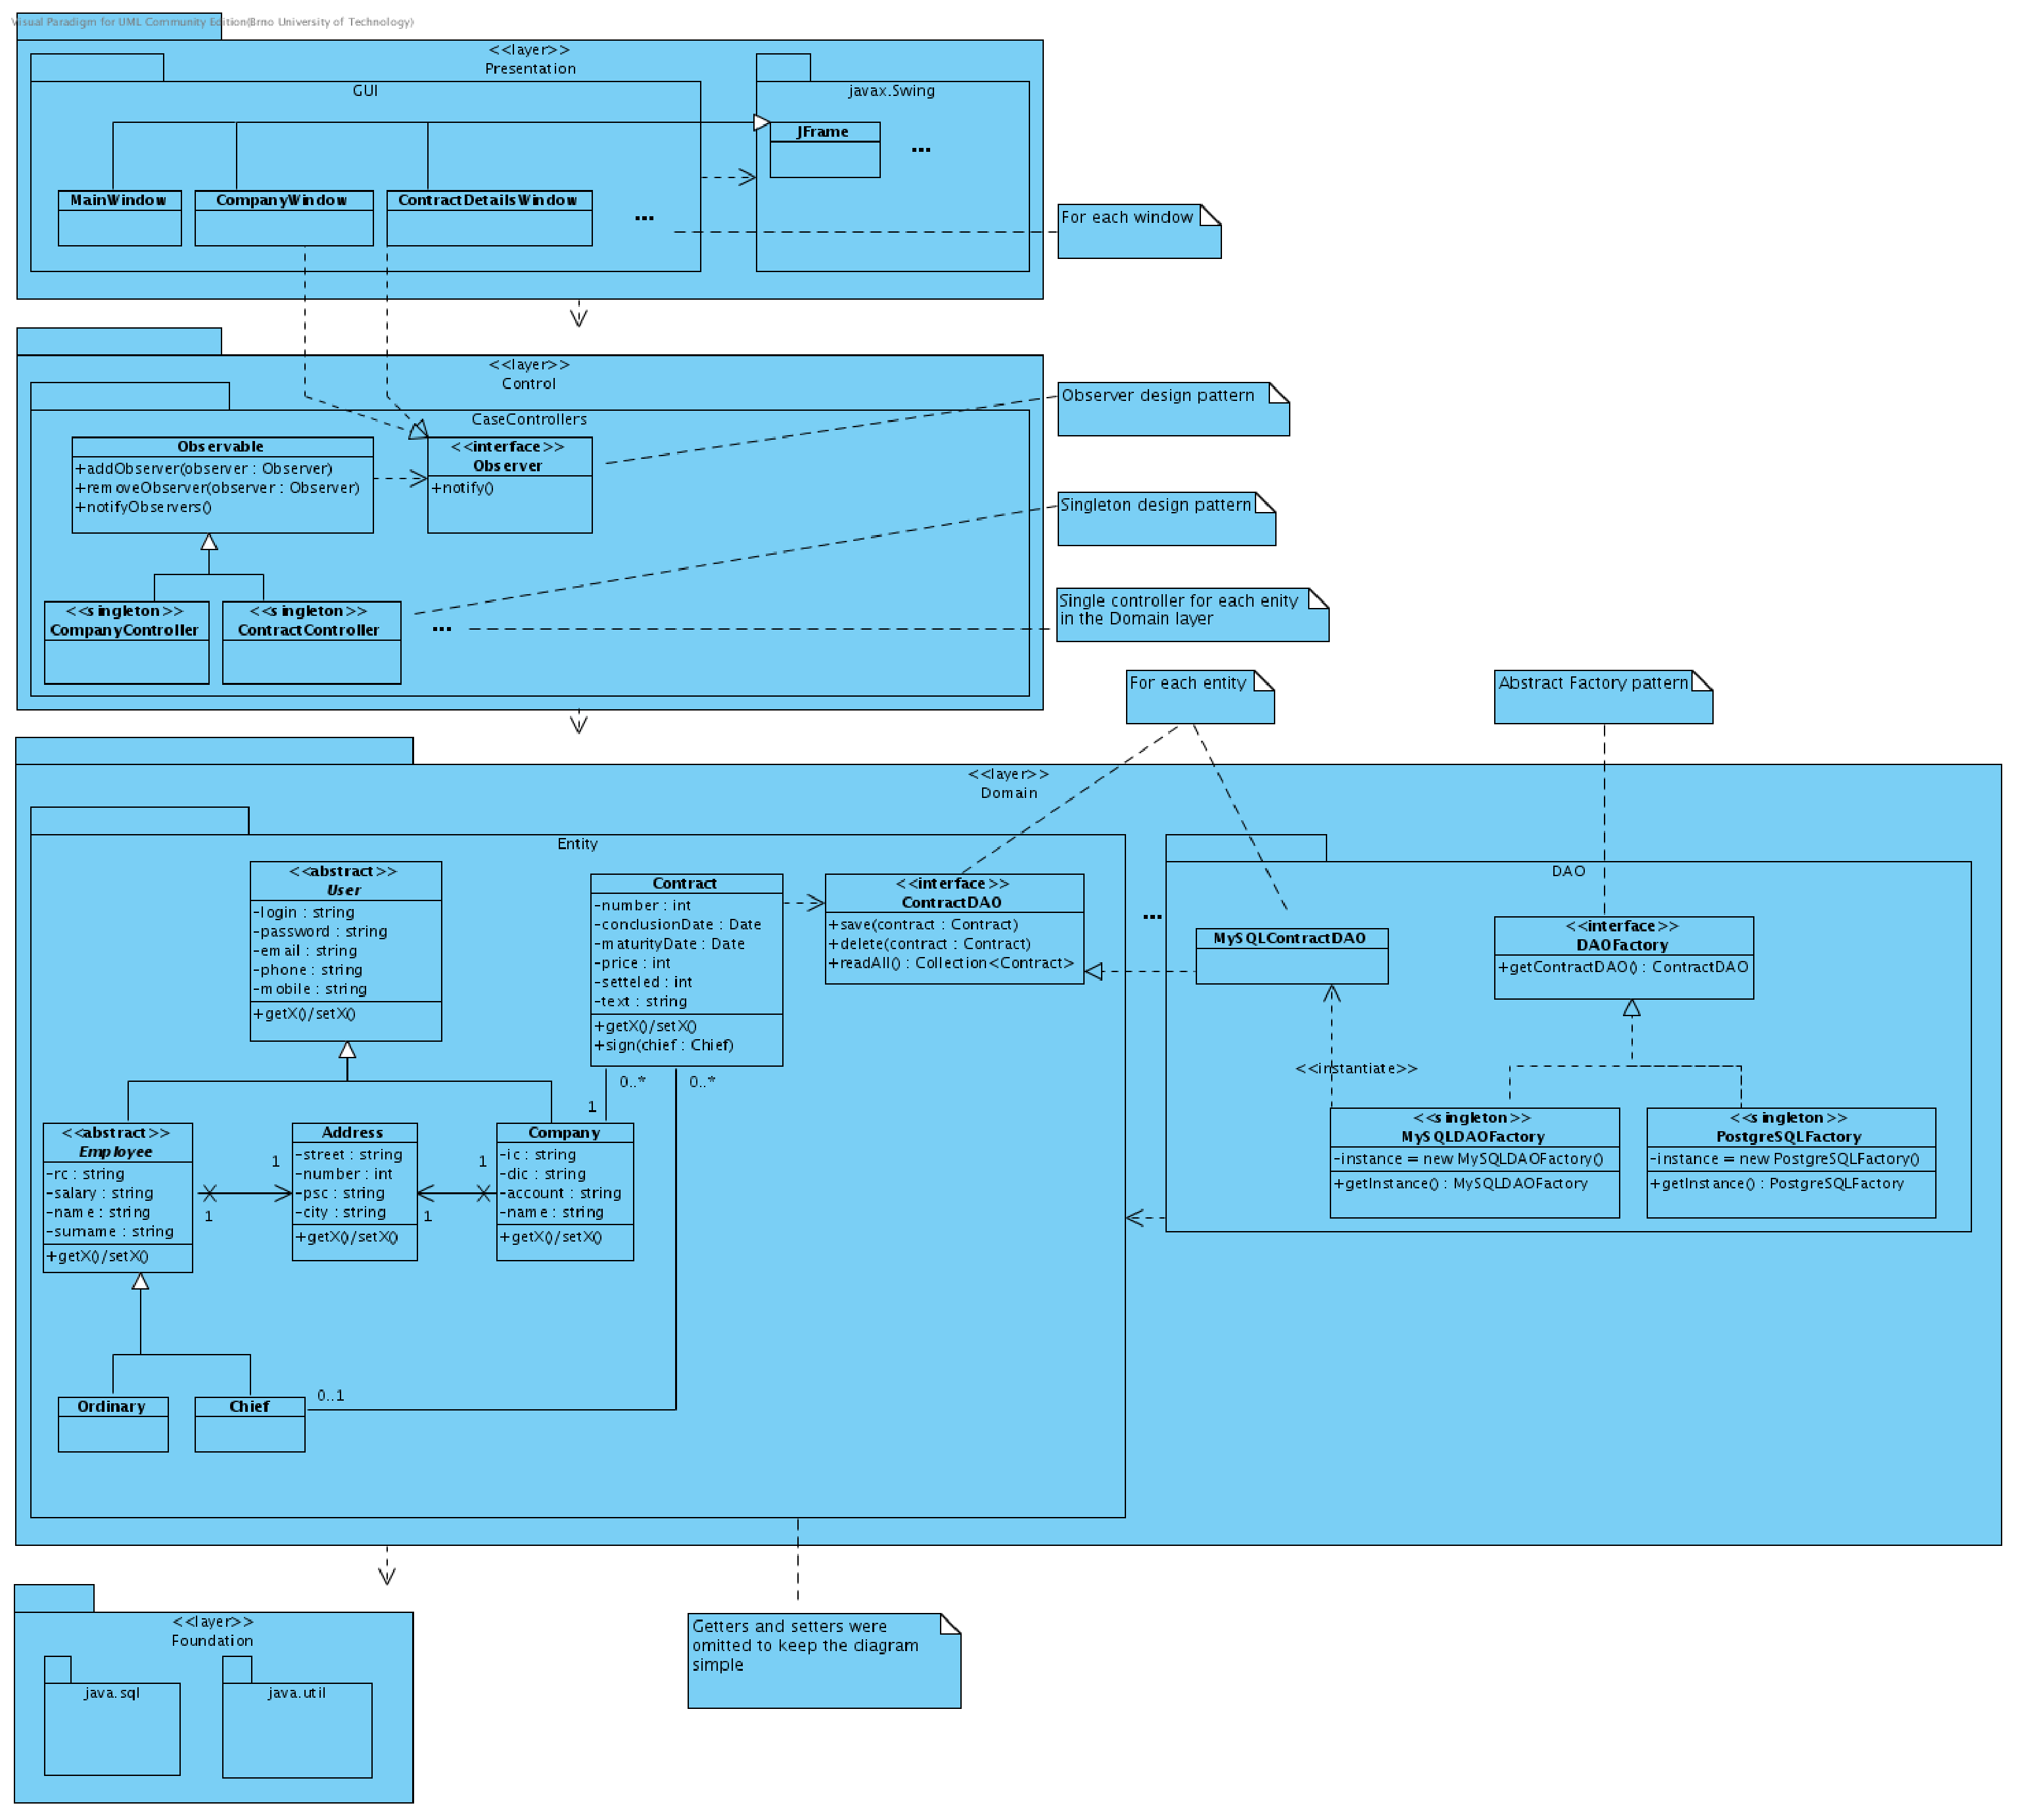
\includegraphics[width=16cm,keepaspectratio]{include/class_stage1}
	\end{center}
	\caption{Diagram návrhových tříd}
	\label{fig:ClassStage1}
\end{figure}

\pagebreak

\section*{Diagramy interakce}

\begin{figure}[H]
	\begin{center}
		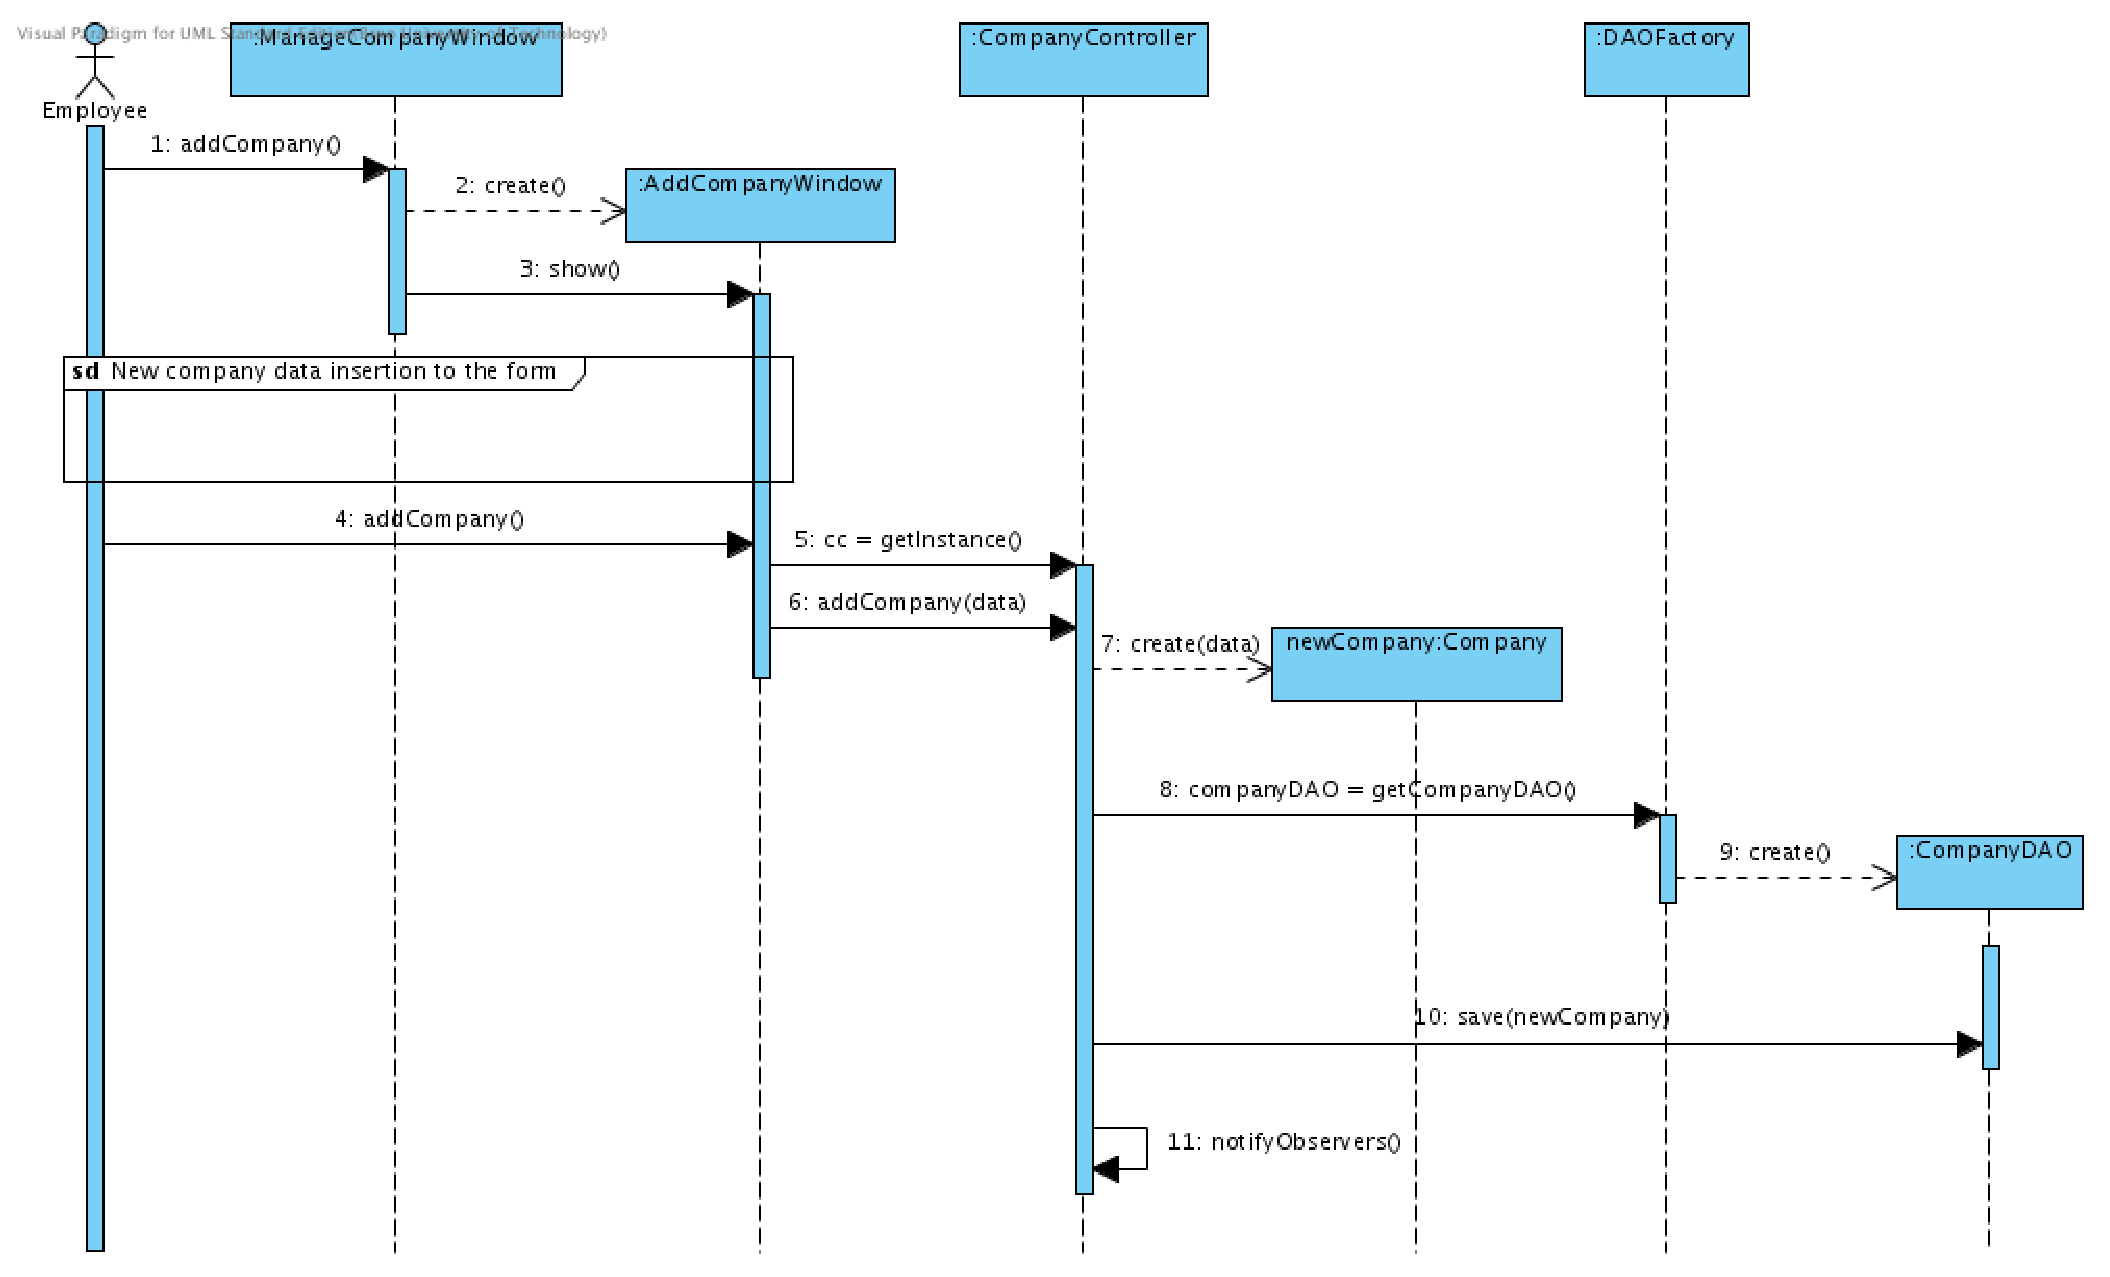
\includegraphics[width=16cm,keepaspectratio]{include/seq_add_company}
	\end{center}
	\caption{Diagram sekvence k~případu použití \uv{Přidat firmu}}
	\label{fig:SeqAddCompany}
\end{figure}

\pagebreak

\begin{figure}[H]
	\begin{center}
		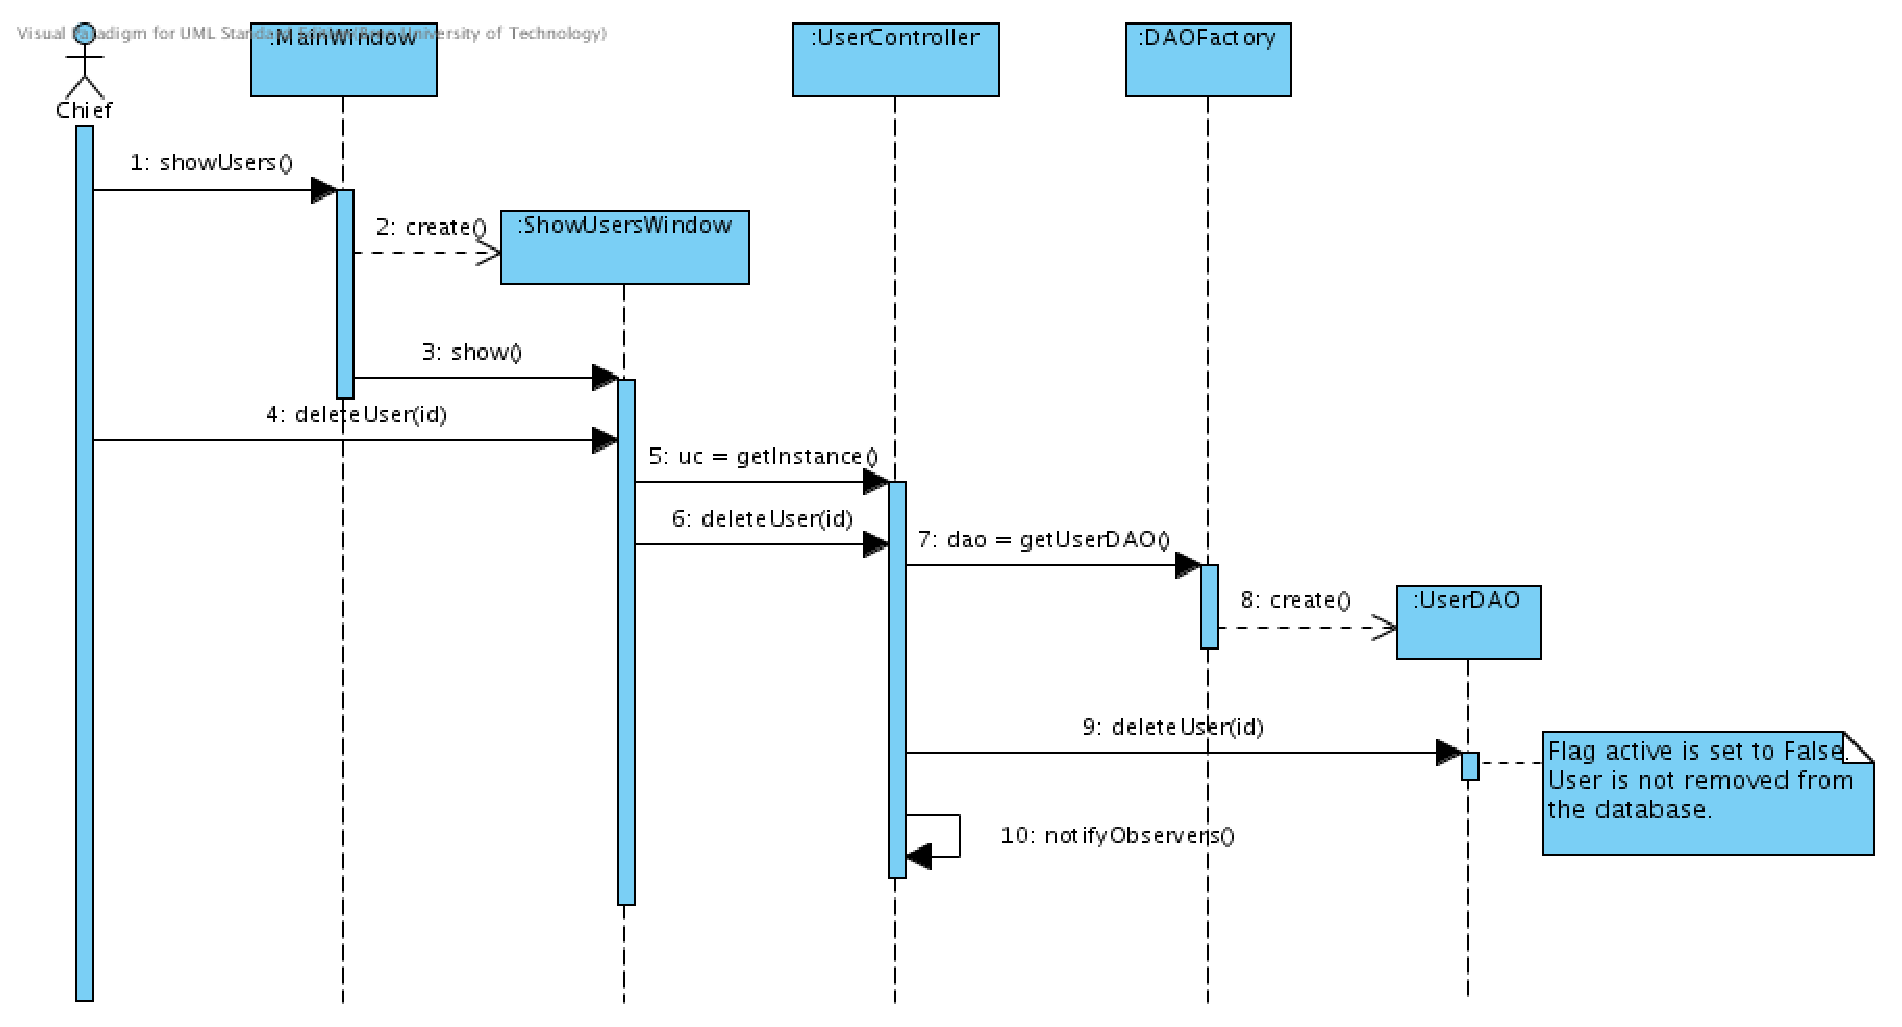
\includegraphics[width=13cm,keepaspectratio]{include/seq_delete_user}
	\end{center}
	\caption{Diagram sekvence k~případu použití \uv{Zrušit zaměstnance}}
	\label{fig:SeqRemoveEmployee}
\end{figure}

%%%%%%%%%%%%%%%%%%%%%%%%%%%%%%%%%%%%%%%%%%%%%%%%%%%%%%%%%%%%%%%%%%%%%%%%%%%%%%%
% vim: syntax=tex
%%%%%%%%%%%%%%%%%%%%%%%%%%%%%%%%%%%%%%%%%%%%%%%%%%%%%%%%%%%%%%%%%%%%%%%%%%%%%%%
